\documentclass[pdftex,10pt,a4paper,oneside]{article}

\usepackage{amsmath} 				%For both in-line and equation mode
\numberwithin{equation}{section} 	%Numbering of our equations per section
\usepackage{algorithm}
\usepackage{algorithmic} 			%Algorithm styles, need to be nested for the example shown
\usepackage{fancyhdr} 				%For our headers
\usepackage{graphicx} 				%Inserting images
\usepackage{lipsum}  				%Blank text fill, delete me when finished
\usepackage{setspace} 				%Spacing on the front page for crest and titles
\usepackage[]{fncychap} 			% Styles can be Sonny, Lenny, Glenn, Conny, Rejne, Bjarne and Bjornstrup
\usepackage[hyphens]{url} 			%Deals with hyphens in urls to make them clickable
\usepackage{xcolor} 				%Great if you want coloured text
\usepackage{tabularx}
\usepackage{appendix} 				%Take a wild guess slick
\usepackage[hidelinks]{hyperref}

\fancyhf{}
\pagestyle{fancy}
\renewcommand{\headrulewidth}{0.2pt}

\begin{document}

% !TEX root =  ../Report.tex

\thispagestyle{empty}

\begin{spacing}{2}
\begin{center}
		\textbf{\begin{LARGE}
بسمه تعالی		
				\end{LARGE}}
		\vspace{10mm}
	\end{center}

	\begin{center}
		
\includegraphics[scale = 0.65]{figs/index.png}
	\end{center}
	
	\vspace{5mm}
	\begin{center}
		\textbf{\begin{LARGE}
		نام گزارش
		\end{LARGE}}
		\vspace{5mm}
	\end{center}
	
	\begin{center}
		{\large 
		توضیحی در مورد عنوان
		}\\
		\vspace{20mm}
	\end{center}
	
	\begin{center}
		\textbf{\large 
نام نگارنده یا نگارنده‌ها		
		}
		\vspace{20mm}
	\end{center}
	
	\begin{center}
	     {\large 
	     استاد راهنما: ...
	      }\\
		\textbf{\large 
دانشکده ...		
		}\\
		{\large 
		توضیح دیگر: ...
		}\\
		{\large 
اطلاعات زمانی (مثلا تابستان ۱۴۰۱)		
		\\}
	\end{center}
	
\end{spacing}

\pagenumbering{roman}



\section*{چکیده}
% سطر بعدی برای آمدن چکیده در فهرست است. به نظرم کار مناسبی نیست.
%\addcontentsline{toc}{section}{چکیده}
\vspace{2cm}

\large
قالب حاضر، برای تسهیل در نگارش متن در بستر
\lr{LaTeX}
تهیه شده است. 
در هر فصل، آموزش فارسی یک سری از کارهای
\lr{LaTeX}
ارائه شده است. در واقع متن این سند شامل مجموعه‌ای از توصیه‌ها است. اما آموزش اصلی با رجوع شما به اسکریپت تولیدکننده هر بخش از متن انجام می‌گیرد. به این ترتیب، با رفتن به سراغ هر یک از فصل‌های مربوطه، در متن فارسی توصیه‌هایی کارآ را می‌خوانید و در کد
\lr{compile}
شده به فرمت «
\lr{.tex}
»، مواد لازم برای ایجاد فصل‌بندی، فهرست‌های مختلف، قراردادن اشکال و جداول و ... را می‌یابید. به قسمت‌های مختلف این نوشتار رجوع کنید و اسکریپت هر قسمت را ببینید تا نحوه انجام کار مربوطه دستتان بیایبد. به عنوان مثال، این قسمت مربوط به چکیده است.
در اینجا چکیده متن در حدود ۳۰۰ کلمه نوشته می شود. 
\\

\vspace{2cm}

\noindent \textit{
 کلمات کلیدی:
 کلمه ۱,
  کلمه ۲,
  کلمه ۳}
\section*{Acknowledgements}
\addcontentsline{toc}{section}{Acknowledgements}

\vspace{2cm}

\large

Always good to acknowledge people. %(yes, there are definitely people to acknowledge )
%Comment the whole thing out if you don't want it

\section*{Abbreviations}
\addcontentsline{toc}{section}{Abbreviations}
\large 
Flux Capacitor \hfill FC\\
Gigawatt \hfill GW\\



\tableofcontents

% Once you start inserting figures, tables and algorithms then they % will start appearing here in the lists. 
%
% The captions and names you give them will appear here. The 
% numbering can either be:
%
%     Natural (1,2,3,...) 
%     Sectional (1.1, 1.2 for chapter 1. 2.1, 2.2,... for chapter 2) 



\listoffigures
\addcontentsline{toc}{section}{List of Figures}
\numberwithin{figure}{section}

\listoftables
\addcontentsline{toc}{section}{List of Tables}
\numberwithin{table}{section}

%Delete me if you're not putting algorithms in or you don't want it as contents. Same applies with the two above ^
\listofalgorithms
\addcontentsline{toc}{section}{List of Algorithms}
\numberwithin{algorithm}{section}

\newpage


\pagenumbering{arabic}

\lfoot{\centering \thepage}



% !TEX root =  ../Report.tex

\section{Introduction}
\label{sec:Introduction} 
%To make a call to the introduction, put \ref{sec:Introduction}. Overleaf can auto-fill it for you

\lipsum[1]
\chapter{ نمونه‌هایی از قراردادن اشکال}
\label{chap:chap2}

در این قسمت، سعی کردم آنچه برای آوردن تصاویر لازم است را فراهم کنم. 
توجه داشته باشید که متداول است که یک پوشه برای عکس‌ها ساخته می‌شود تا فایل‌ها نظم و ترتیب بهتری داشته باشند. من در تهیه این قالب یک پوشه
\lr{'figs'}
درست کرده‌ام و همه عکس‌ها را در آن قرار داده‌ام. توجه داشته باشید که اسم و آدرس هر عکس است که در ترسیم آن مهم است.
آوردن تصویرهای تکی و شکل‌های دسته‌ای را جداگانه آورده‌ام.

\section{
شکل با یک تصویر تکی
}

شکل
\ref{fig:clock_tower_photo}
یک نمونه است. به اسکریپت مربوط به آن دقت کنید و سعی کنید معنی هر دستور را بفهمید تا بتوانید در صورت تمایل، در گزارش خودتان تغییرات لازم را ایجاد کنید. در غیر اینصورت، این یک نمونه عادی از آوردن شکل در متن است که می‌توانید مستقیما از آن استفاده کنید.

\begin{figure}[h]
    \centering
    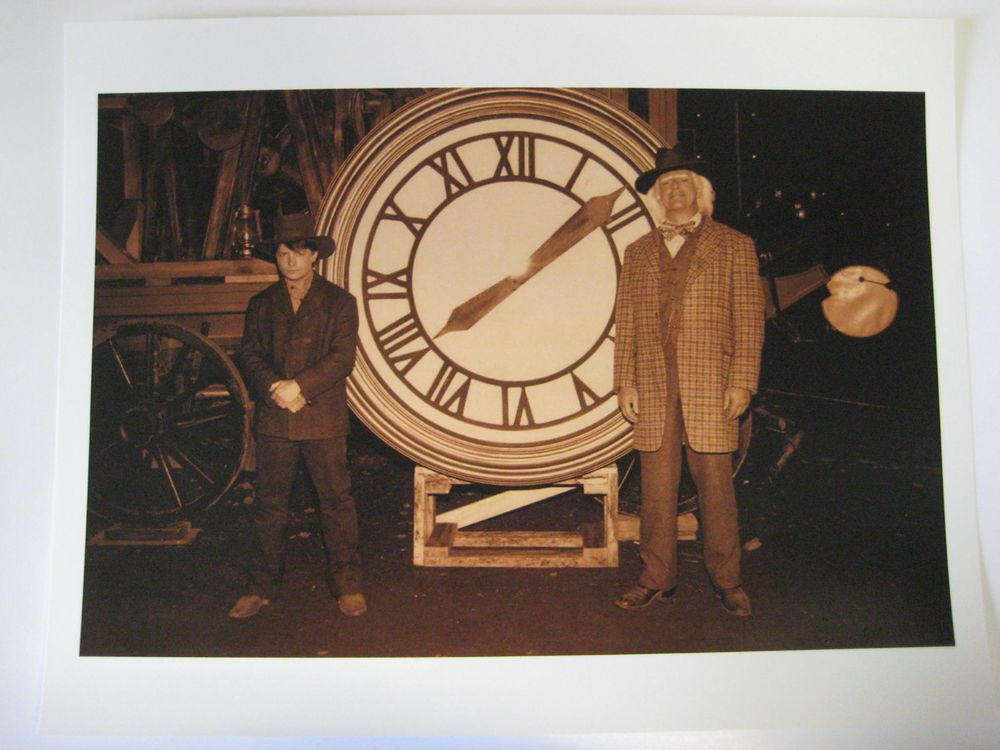
\includegraphics[width=0.5\textwidth]{figs/doc_and_marty.jpg}
    \caption{
    توضیح زیر عکس
    }
    \label{fig:clock_tower_photo}
\end{figure}


\section{
شکل با چند عکس داخل آن
}


یک نمونه از تصویر با چند عکس داخل آن:


\begin{figure}[h]
\centering
\subfigure[نمای آغاز]{
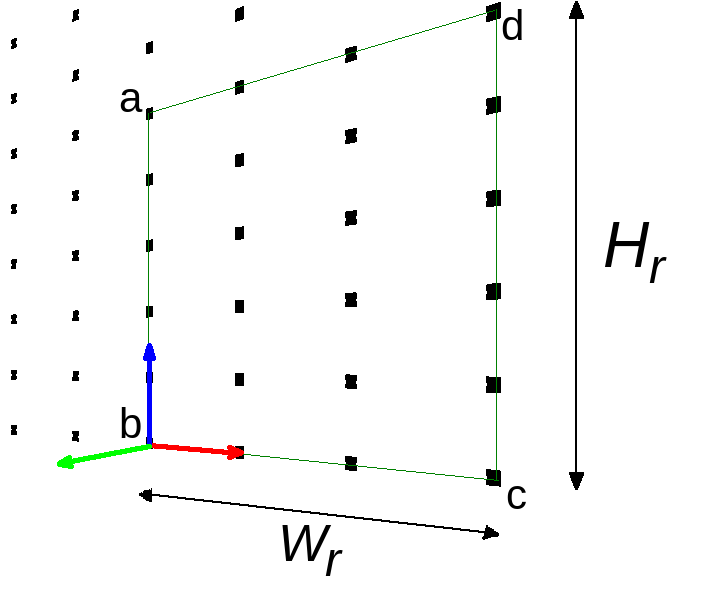
\includegraphics[width=0.3\linewidth]{figs/poor_view.png}
	\label{fig:poor_view}
}
\hspace*{15mm}
\subfigure[نمای پایان]{
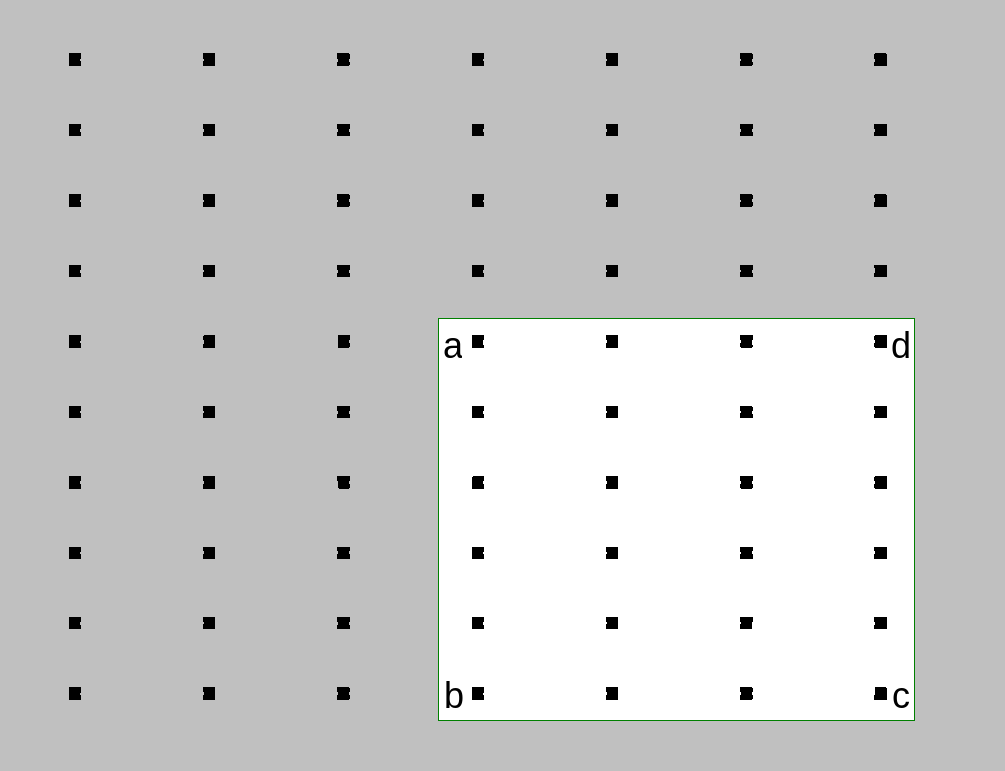
\includegraphics[width=0.3\linewidth]{figs/exact_view.png}
	\label{fig:exact_view}
}

\caption{نمای دوربین ریزپرنده در آغاز و پایان مرحله بهینه‌سازی موقعیت دید}

\label{fig:g1_views}
\end{figure}

یک نمونه دیگر با تعداد عکس بیشتر:

\begin{figure}[ht]
\centering
\subfigure[]{
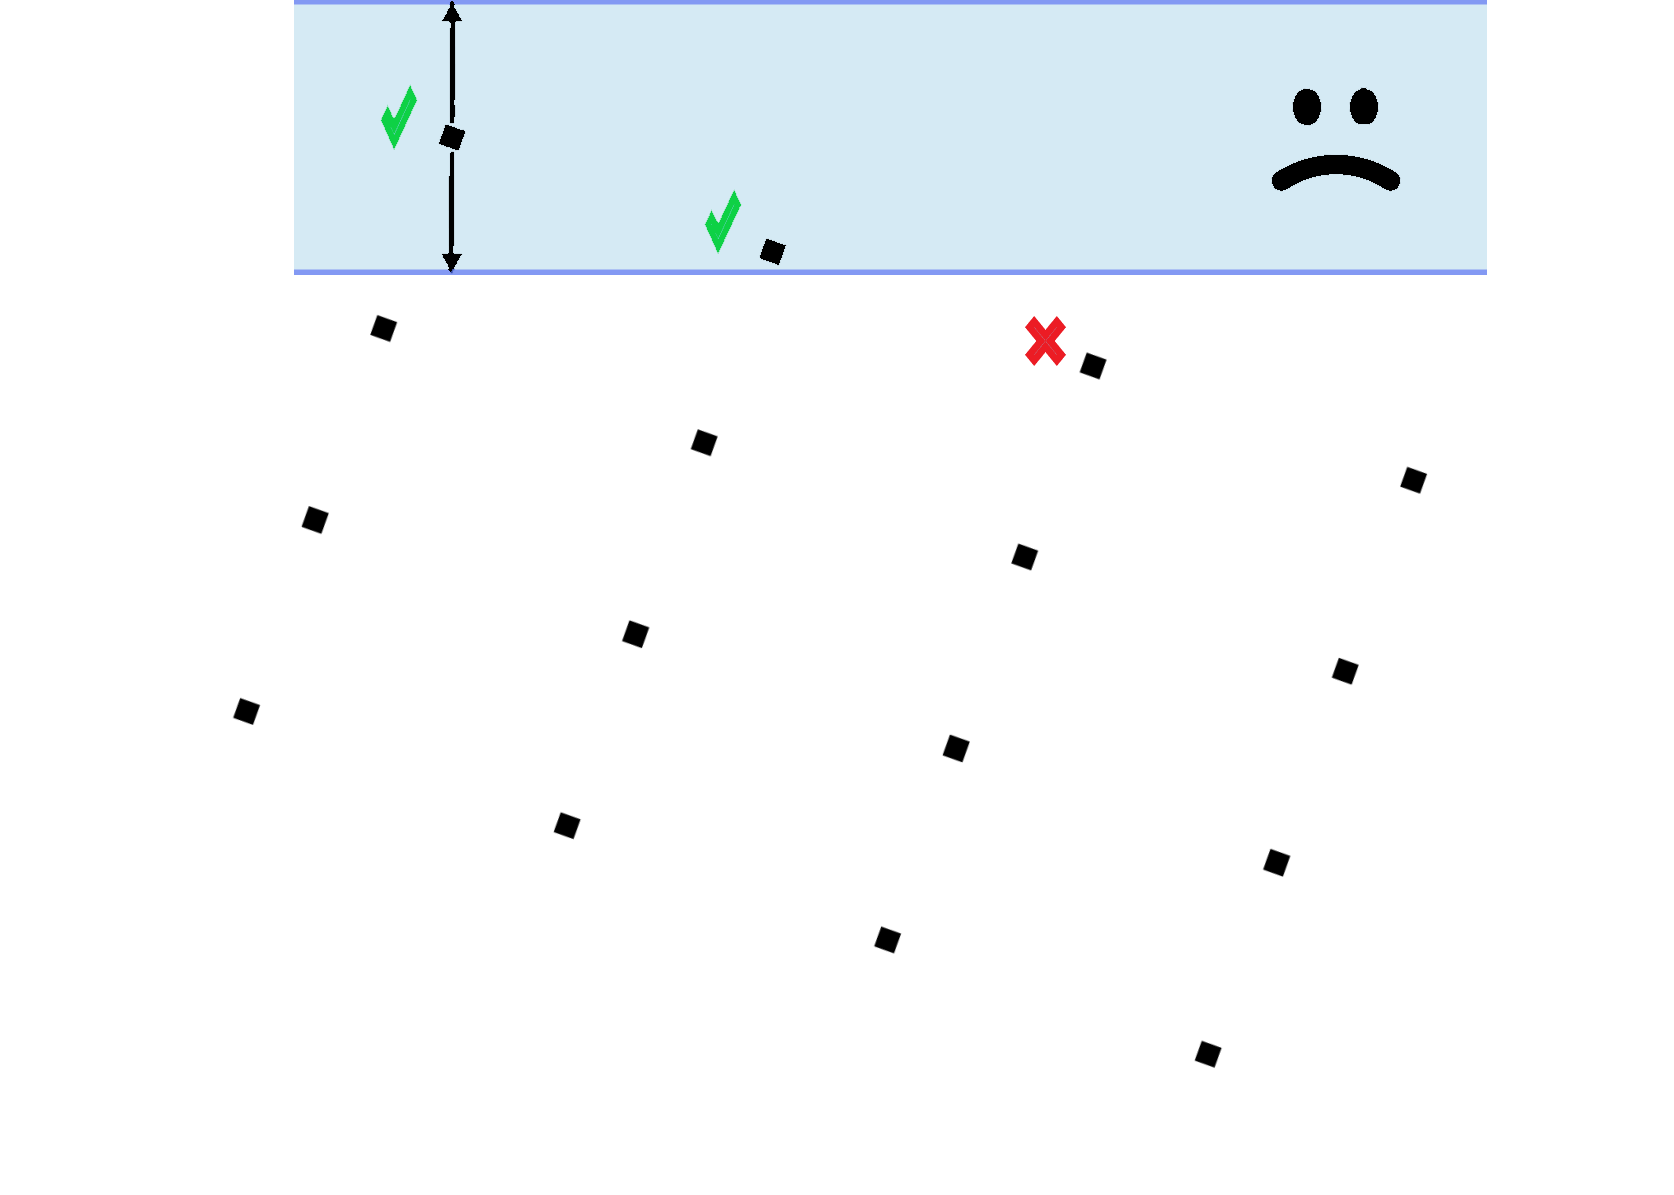
\includegraphics[width=0.3\linewidth]{figs/algorithm1.png}
	\label{fig:sc_vis_algorithm1}
}
\hspace*{1mm}
\subfigure[]{
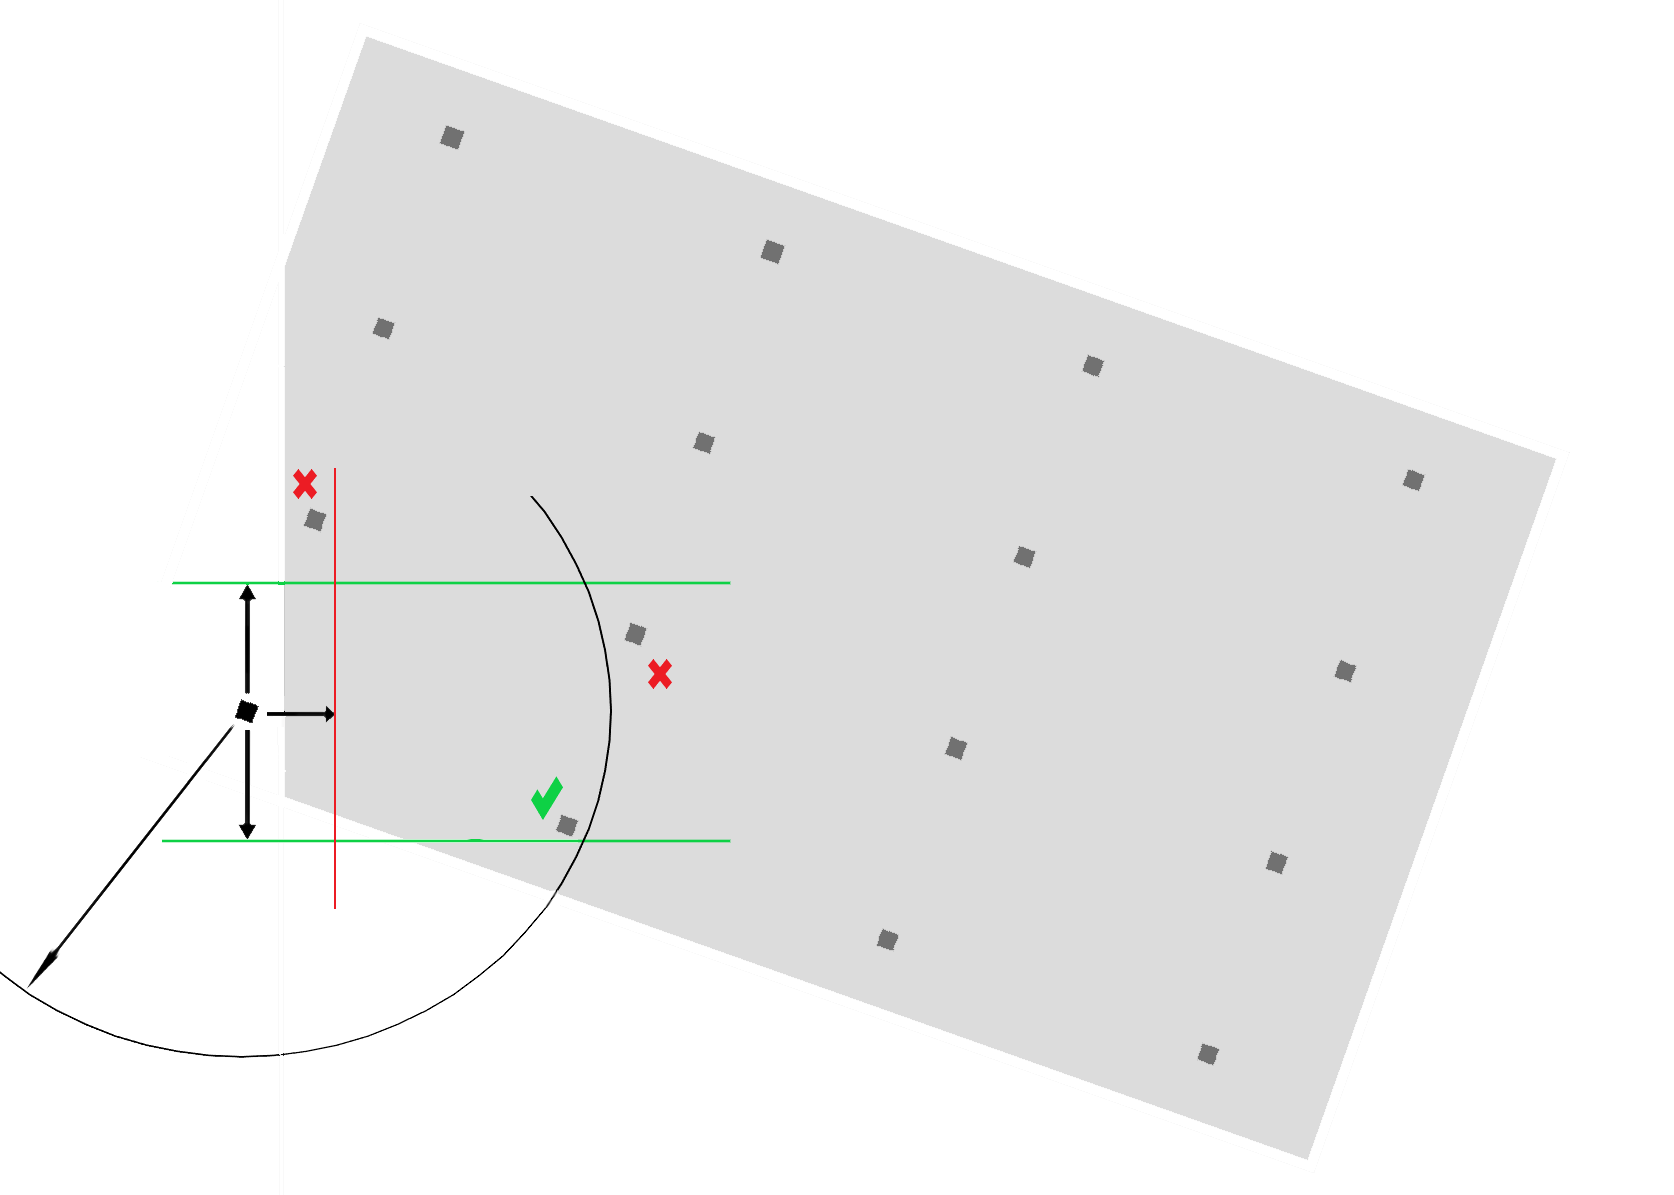
\includegraphics[width=0.3\linewidth]{figs/algorithm2.png}
	\label{fig:sc_vis_algorithm2}
}
\hspace*{1mm}
\subfigure[]{
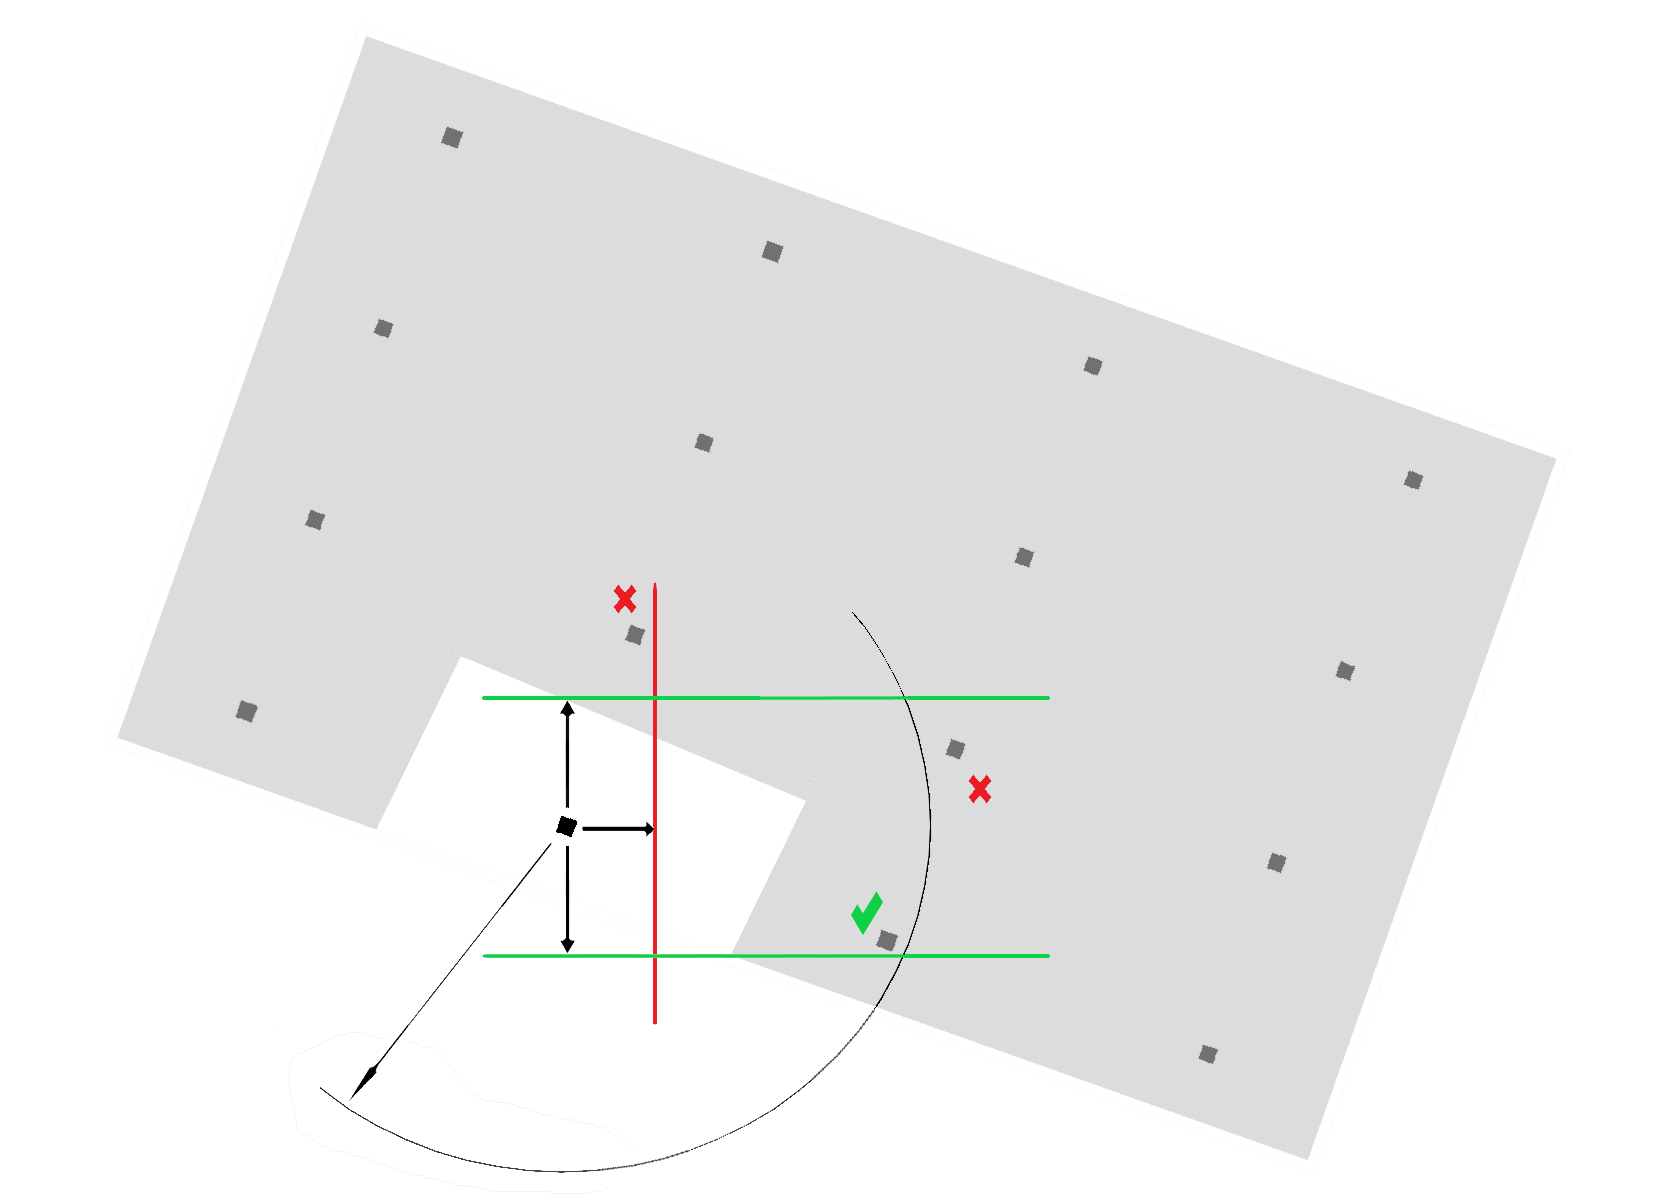
\includegraphics[width=0.3\linewidth]{figs/algorithm3.png}
	\label{fig:sc_vis_algorithm3}
}
\hspace*{1mm}
\subfigure[]{
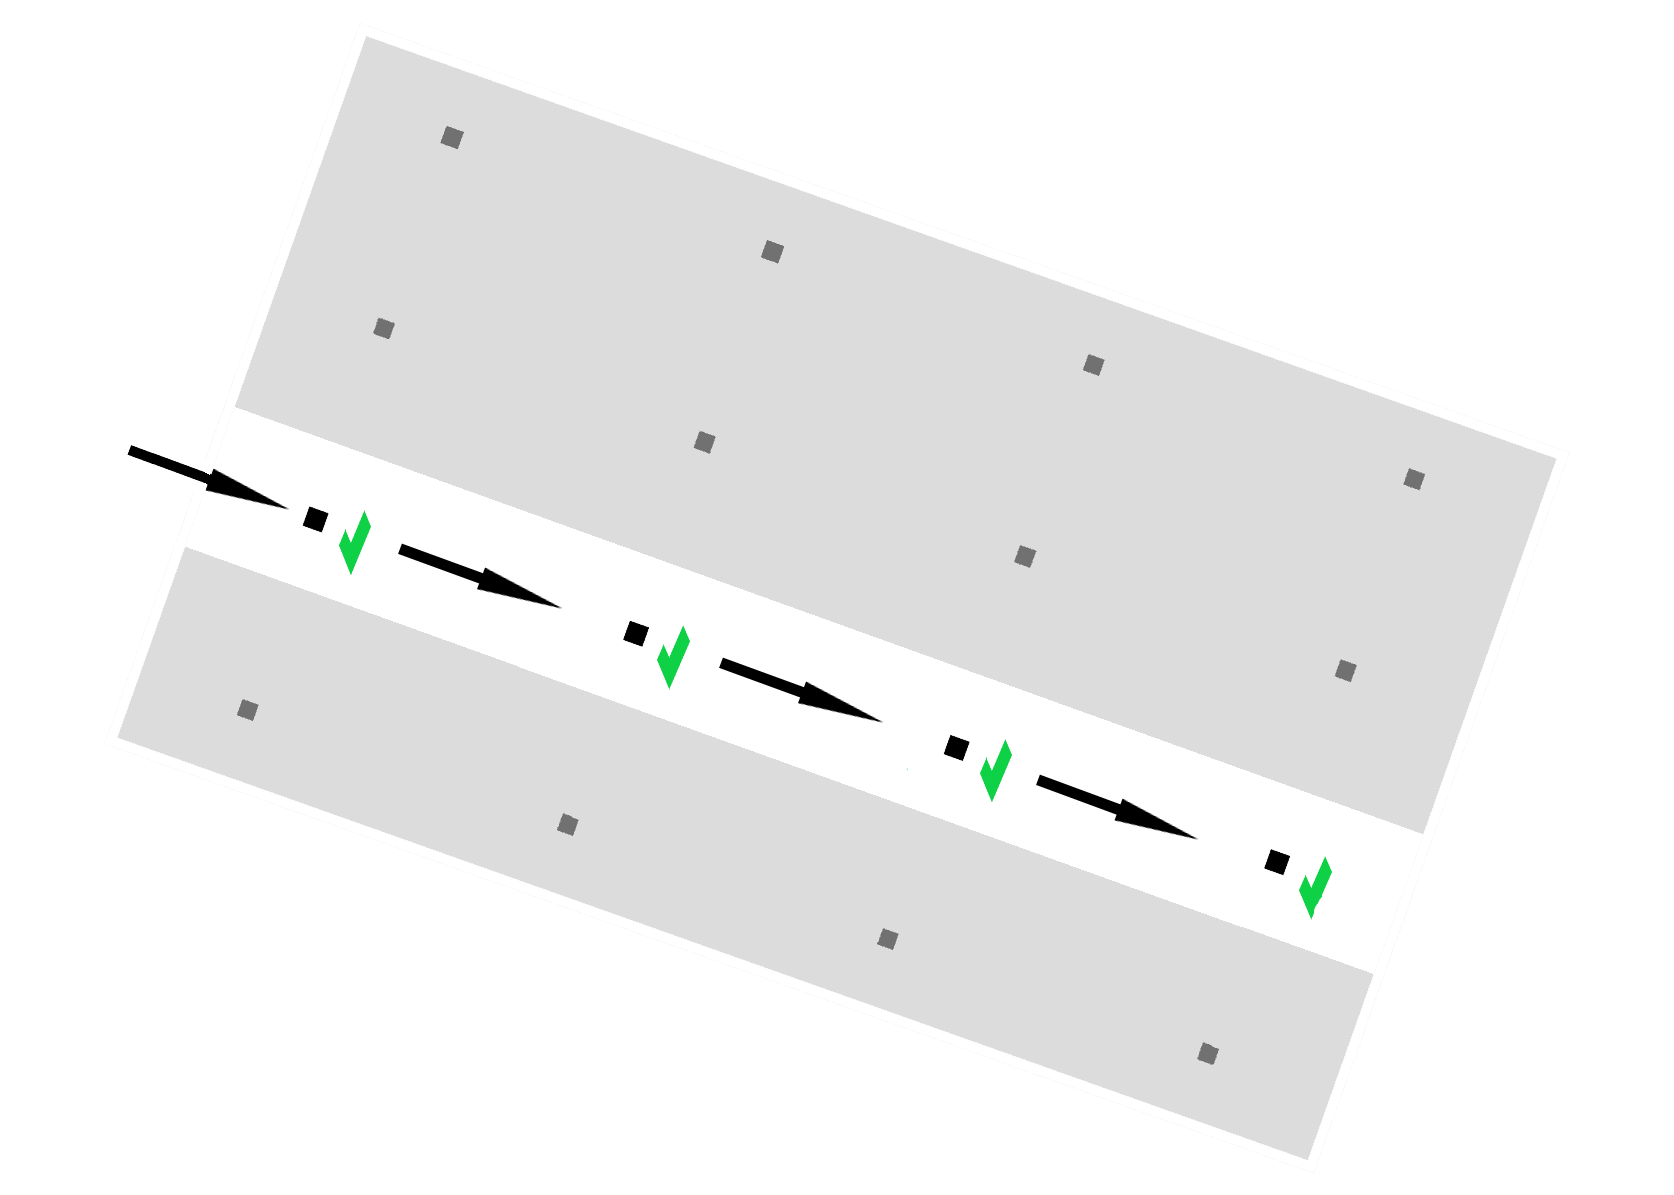
\includegraphics[width=0.3\linewidth]{figs/algorithm4.png}
	\label{fig:sc_vis_algorithm4}
}
\hspace*{1mm}
\subfigure[]{
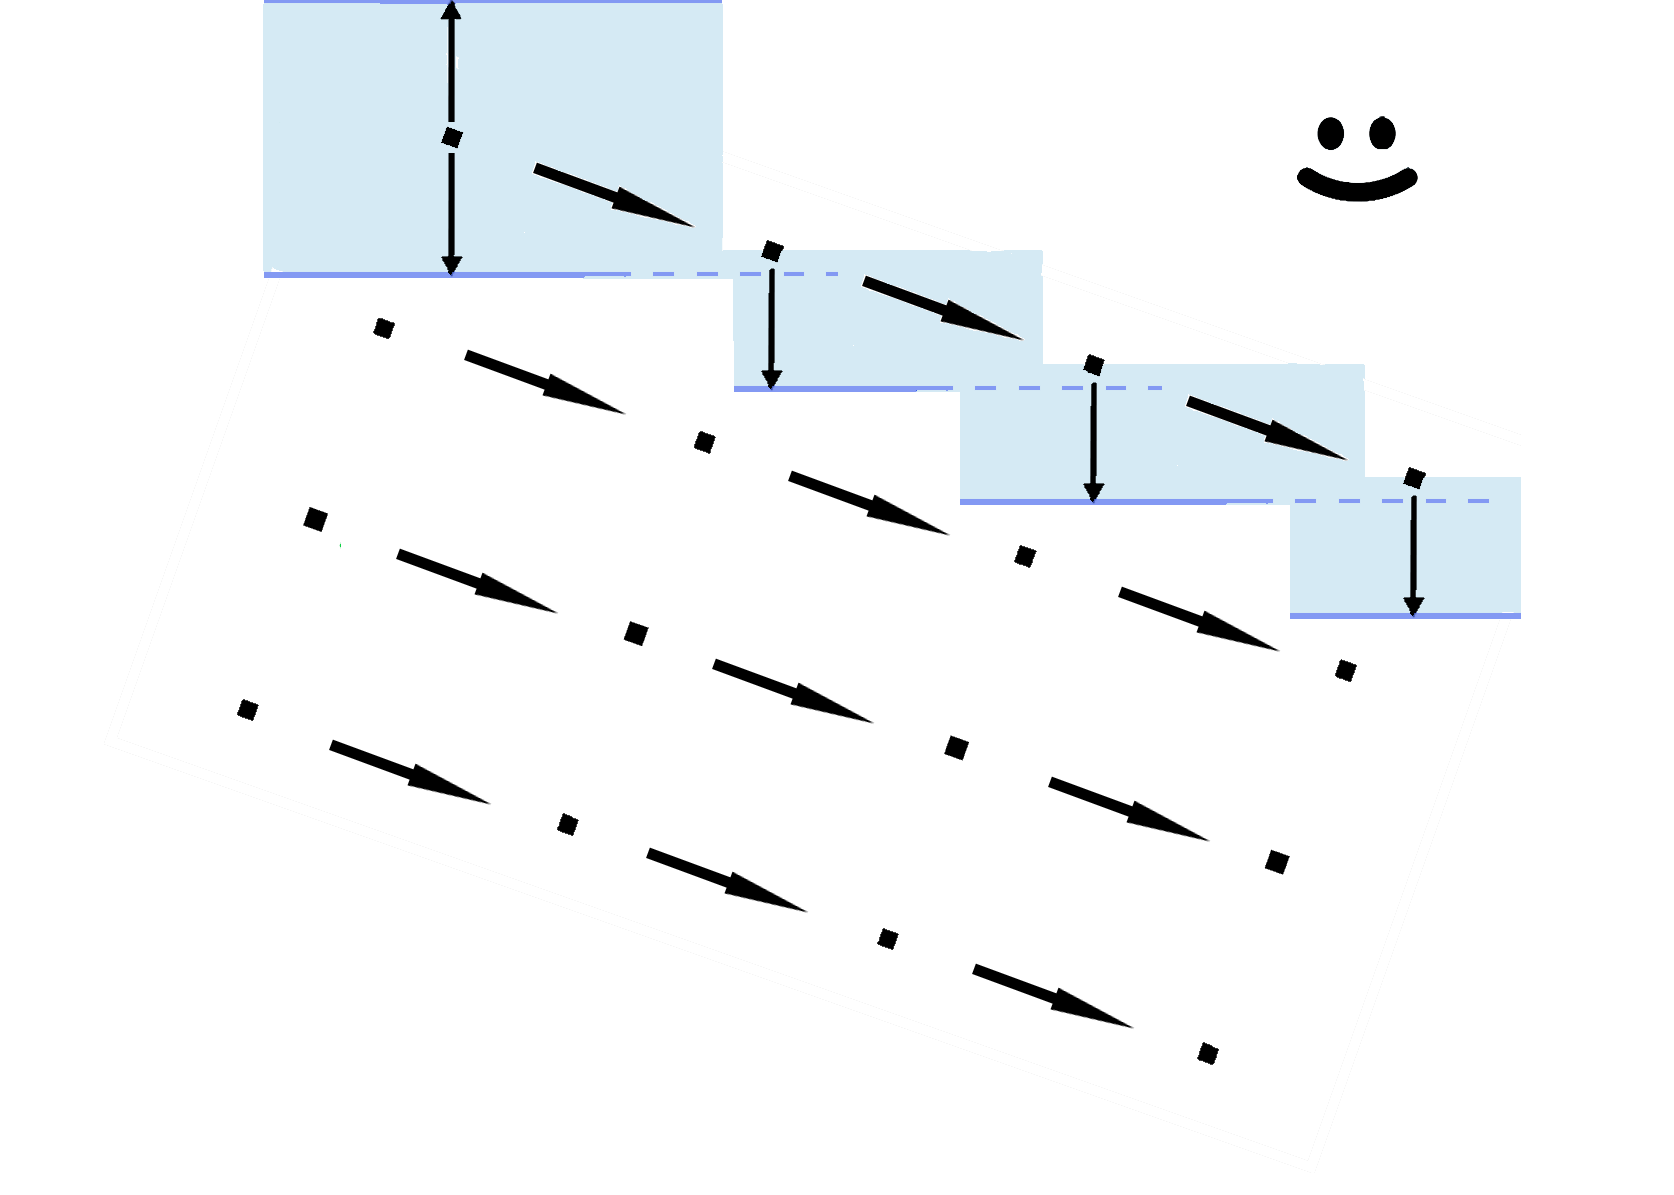
\includegraphics[width=0.3\linewidth]{figs/algorithm5.png}
	\label{fig:sc_vis_algorithm5}
}

\caption{
نمایی از مراحل پردازش داده جدول نقاط در روش دسته‌بندی پله‌ای
}
\label{fig:sc_algorithm}
\end{figure}
\chapter{
جداول در
\lr{LaTeX}
}
\label{chap:chap3}

شاید طراحی جدول در
\lr{LaTeX}
جزو کارهای سخت به نظر برسد. البته در حقیقت اینطور نیست. اگر شما روی این نظر مصر هستید و در این زمینه
\lr{LaTeX}
را با نرم افزارهای ویرایش متن
\lr{microsoft}
مقایسه می‌کنید، باید به شما بادآوری کنیم که هر چه یک رابط گرافیکی کارتان را راحت کند، به همان میزان برای شما تصمیم می‌گیرد و شما را از یک «توسعه‌دهنده» بودن، به سمت یک یک «کاربر عادی» بودن سوق می‌دهد.

در این متن، من کارهایی که باید بکنید تا در
\lr{LaTeX}
جدول درست شود را توضیح نمی‌دهم. خودتان اسکریپت‌ها را ببینید تا بفهمید. اما اولین توصیه من برای طراحی جدول، همان چیزی است که در قسمت
\ref{sec:text} 
گفتم. سعی کنید در
\lr{LaTeX}
، چه فارسی چه انگلیسی، هر دستور را در یک سطر مجزا بنویسید. آن موقع خواهد فهمید که سخت‌ترین کارها چقدر آسان می‌شود. باید توجه کنید که وقتی با
\lr{LaTeX}
متن می‌نویسید، شما در واقع به همان میزان که دارید تولید محتوی می‌کنید، دارید کد هم می‌زنید! و خوب اگر یک برنامه‌نویس باشید، می‌دانید که جدای از الگوریتمی که اجرا می‌شود، نجوه نگارش متن برنامه چقدر مهم است؛ و چقدر در فهم و راحت‌شدن کار کمک می‌کند. 

جدول
\ref{tab:inventory}
یک نمونه برای شما است. نگاه کنید که آن را چطور نوشته‌ام. سعی کنید خوب فرق عملگرهای مربوط به سطر جدید یا ستون جدید را بفهمید.


\begin{table}[H] 
\caption{کپشن برای جدول}
\label{tab:inventory}
\begin{tabularx}{\textwidth}{| X | X |}
    \hline
     مورد
      & 
      توضیح
        \\ \hline
      
     مورد ۱
     & 
     توضیح ۱ 
     \\ \hline
     
     مورد ۲ 
     & 
     توضیح ۲ 
     \\ \hline
     
     مورد ۳ 
     & 
     توضیح ۳
     \\ \hline
     
\end{tabularx}
\end{table}


یک حقه ساده دیگر که البته این یکی را اگر تا کنون با
\lr{LaTeX}
کار کرده باشید به احتمال زیاد می‌دانید. می‌توانید برای راحتی در طراحی جدول، از وبگاه‌هایی که به صورت رایگان و با رابط گرافیکی اسکریپت
\lr{LaTeX}
مربوط به جدول دلخواه شما را تولید می‌کنند استفاده کنید. خیلی ساده است. کافی است عبارت زیر را در گوگل جستجو کنید:

\begin{flushleft}
\lr{latex table online}
\end{flushleft}

یک جدول نمونه دیگر:

\begin{table}[!ht]
\caption{
اطلاعات مربوط به قفسه‌ها و انبار شبیه‌سازی‌شده
}
\label{tab:sim_shelf_info}
\centering
\begin{tabular}{|c|c|}
\hline
مولفه                     & اندازه \\ \hline
ابعاد آرایه سلول‌های قفسه &    6 × 10    \\ \hline
ابعاد کل قفسه             &  \lr{m} 0.4 × \lr{m} 3.77 × \lr{m} 3.5 \\ \hline
ابعاد هر سلول             &  \lr{cm} 40 × \lr{cm} 57 × \lr{cm} 30 \\ \hline
ابعاد برچسب‌های رنگی      &  \lr{cm} 5 × \lr{cm} 5 \\ \hline
ابعاد نشانگرها            & \lr{cm} 10 × \lr{cm} 10 \\ \hline
فاصله میان دو قفسه متوالی &  \lr{m} 3 \\ \hline
تعداد کل قفسه‌ها          &   5   \\ \hline
\end{tabular}
\end{table}

\section{Making a reference}
\label{sec: Reference}

\noindent In this chapter we shall do a reference to an entry in the bibliography, \texttt{bibliography.bib}. \\

What we know of the invention of the flux capacitor is that Dr. Emmett Brown thought of this when hanging a clock in the bathroom. He was standing on his porcelain sink and slipped because it was wet, the resulting hit on the head was apparently a cause to this invention \cite{example}.\\

The corresponding sketch made on this day has been attached in appendix \ref{appx: Flux Sketch}.



\bibliographystyle{abbrv}
\bibliography{bibliography}

\begin{appendices}
\addcontentsline{toc}{section}{Appendices}


\section{The Flux Sketch}
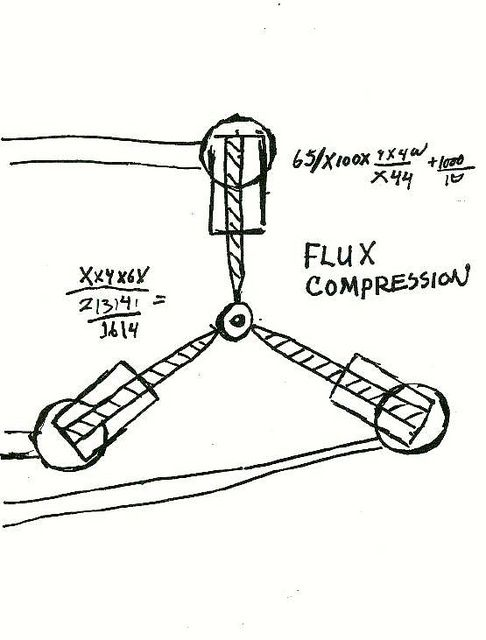
\includegraphics[width=\textwidth]{fig/flux_sketch.jpg}
\label{appx: Flux Sketch}



\end{appendices}

\end{document}
